\documentclass[12pt,t]{beamer}
\usepackage{graphicx}
\setbeameroption{hide notes}
\setbeamertemplate{note page}[plain]
\usepackage{listings}

% set up listing environment
\lstset{language=bash,
        basicstyle=\scriptsize,
        frame=single,
        backgroundcolor=\color{darkgray},
        commentstyle=\color{green},
        showspaces=false,
        showstringspaces=false
        }

% get rid of junk
\usetheme{default}
\beamertemplatenavigationsymbolsempty
\hypersetup{pdfpagemode=UseNone} % don't show bookmarks on initial view


% font
\usepackage{fontspec}
\setsansfont{TeX Gyre Heros}
\setbeamerfont{note page}{family*=pplx,size=\footnotesize} % Palatino for notes
% "TeX Gyre Heros can be used as a replacement for Helvetica"
% In Unix, unzip the following into ~/.fonts
% In Mac, unzip it, double-click the .otf files, and install using "FontBook"
%   http://www.gust.org.pl/projects/e-foundry/tex-gyre/heros/qhv2.004otf.zip

% named colors
\definecolor{offwhite}{RGB}{249,242,215}
\definecolor{foreground}{RGB}{255,255,255}
\definecolor{background}{RGB}{24,24,24}
\definecolor{title}{RGB}{107,174,214}
\definecolor{gray}{RGB}{155,155,155}
\definecolor{subtitle}{RGB}{102,255,204}
\definecolor{hilight}{RGB}{102,255,204}
\definecolor{vhilight}{RGB}{255,111,207}
\definecolor{nhilight}{RGB}{128,0,128}  % hilight color in notes
\definecolor{nvhilight}{RGB}{255,0,128} % vhilight for notes
\definecolor{lolight}{RGB}{155,155,155}
%\definecolor{green}{RGB}{125,250,125}

% use those colors
\setbeamercolor{titlelike}{fg=title}
\setbeamercolor{subtitle}{fg=subtitle}
\setbeamercolor{institute}{fg=gray}
\setbeamercolor{normal text}{fg=foreground,bg=background}
\setbeamercolor{item}{fg=foreground} % color of bullets
\setbeamercolor{subitem}{fg=gray}
\setbeamercolor{itemize/enumerate subbody}{fg=gray}
\setbeamertemplate{itemize subitem}{{\textendash}}
\setbeamerfont{itemize/enumerate subbody}{size=\footnotesize}
\setbeamerfont{itemize/enumerate subitem}{size=\footnotesize}

% page number
\setbeamertemplate{footline}{%
    \raisebox{5pt}{\makebox[\paperwidth]{\hfill\makebox[20pt]{\color{lolight}
          \scriptsize\insertframenumber}}}\hspace*{5pt}}

% add a bit of space at the top of the notes page
\addtobeamertemplate{note page}{\setlength{\parskip}{12pt}}

% default link color
\hypersetup{colorlinks, urlcolor={hilight}}

% a few macros
\newcommand{\bi}{\begin{itemize}}
\newcommand{\ei}{\end{itemize}}
\newcommand{\ig}{\includegraphics}
\newcommand{\subt}[1]{{\footnotesize \color{subtitle} {#1}}}
\newcommand{\ttsm}{\tt \small}

%%%%%%%%%%%%%%%%%%%%%%%%%%%%%%%%%%%%%%%%%%%%%%%%%%%%%%%%%%%%%%%%%%%%%%
% end of header
%%%%%%%%%%%%%%%%%%%%%%%%%%%%%%%%%%%%%%%%%%%%%%%%%%%%%%%%%%%%%%%%%%%%%%

% title info
\title{Unix command line; editors}
\subtitle{Tools for Reproducible Research}
\author{\href{http://www.biostat.wisc.edu/~kbroman}{Karl Broman}}
\institute{Biostatistics \& Medical Informatics, UW{\textendash}Madison}
\date{\href{http://www.biostat.wisc.edu/~kbroman}{\tt \scriptsize \color{white} biostat.wisc.edu/{\textasciitilde}kbroman}
\\[-4pt]
\href{http://github.com/kbroman}{\tt \scriptsize \color{white} github.com/kbroman}
\\[-4pt]
\href{https://twitter.com/kwbroman}{\tt \scriptsize \color{white} @kwbroman}
\\[-4pt]
{\scriptsize Course web: \href{http://bit.ly/tools4rr}{\tt bit.ly/tools4rr}}
}


\begin{document}

% title slide
{
\setbeamertemplate{footline}{} % no page number here
\frame{
  \titlepage
  \note{For your work to be reproducible, it needs to be code-based;
    don't touch that mouse!

Some flavor of Unix will be most efficient; you'll want to be
comfortable with command-line tools.

And you'll spend a lot of time using an editor. Learn to use a
powerful one.
}
} }


\begin{frame}[c]{}


\centering
\Large

Windows {\color{lolight} vs.} Mac OSX {\color{lolight} vs.} Linux

\bigskip
\bigskip

Remote {\color{lolight} vs.} Not

\note{The Windows operating system is not very programmer-friendly.

Mac OSX isn't either, but under the hood, it's just unix.

Don't touch the mouse! Open a terminal window and start typing.

I do most of my work directly on my desktop or laptop. You might
prefer to work remotely on a server, instead. But I can't stand having
any lag in looking at graphics.
}
\end{frame}


\begin{frame}[c]{If you're stuck with Windows...}

\centering
\Large

Consider \href{http://www.cygwin.org}{Cygwin}
{\color{lolight} (and perhaps \href{https://code.google.com/p/mintty/}{Mintty})}

\note{Cygwin is an effort to get Unix command-line tools in Windows.

Mintty is a terminal emulator.}
\end{frame}

\begin{frame}[c]{If you use a Mac...}

\centering
\Large

Consider \href{http://brew.sh/}{Homebrew} and
\href{http://www.iterm2.com}{iTerm2}

\note{Homebrew is a packaging system; iTerm2 is a Terminal replacement}

\end{frame}


\begin{frame}{The command line is your friend}

\vspace{24pt}

\bi
\itemsep24pt
\item Don't touch that mouse!
\item Scriptable
\item Flexible
\ei
\note{In the long run, you'll be happier, having conquered the command line.

Pointing-and-clicking is not reproducible, and every time you take
your hands off the keyboard, there's a loss of efficiency.

The command line allows you to piece together multiple tools and so do
things that weren't anticipated by the developer of the GUI.
}
\end{frame}



\begin{frame}[c]{The shell}


\centerline{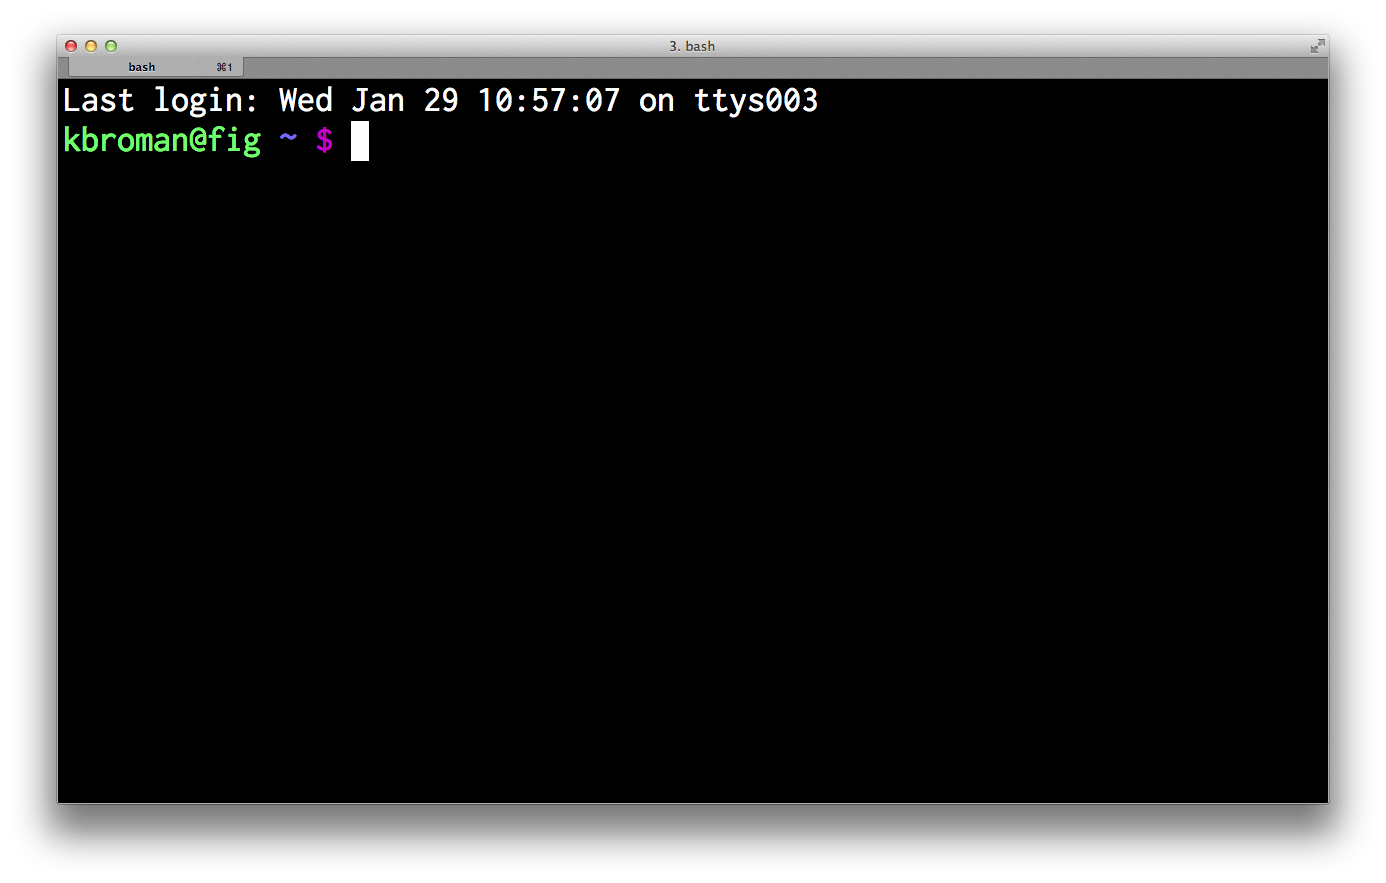
\includegraphics[width=\textwidth]{Figs/shell.png}}

Options: \href{http://en.wikipedia.org/wiki/Tcsh}{tcsh}, \href{http://www.gnu.org/software/bash/manual/bashref.html}{bash}, \href{http://www.zsh.org/}{zsh}


\note{The shell is a program -- an interface to the operating
  system.}

\end{frame}



\begin{frame}{Basics}

\vspace{18pt}
\bi
\itemsep18pt
\item Directory structure

{\color{lolight} Absolute vs. relative paths

\tt ls -l {\textasciitilde}/.. }

\item Creating, removing, changing directories

{\tt \color{lolight} mkdir 

rmdir

cd

cd -}

\item Moving, copying, removing files

{\tt \color{lolight} mv

cp 

rm -i}

\ei

\note{This stuff is too boring to spend much time on.

But I should emphasize the importance of using relative paths (e.g.,
{\tt ../Figs/fig1.pdf}) in a project; reliance on absolute paths
(e.g., {\tt {\textasciitilde}/Projects/Blah/Figs/fig1.pdf}) make life difficult when
you move the project to a different system.
}

\end{frame}


\begin{frame}[fragile]{{\tt {\textasciitilde}/.bash\_profile}}

\vspace{-12pt}

\begin{semiverbatim}
\begin{lstlisting}
export PATH=.:/usr/local/bin:$PATH
export LD_LIBRARY_PATH=/usr/local/lib

noclobber=1    # prevent overwriting of files
IGNOREEOF=1    # disable Ctrl-D as a way to exit
HISTCONTROL=ignoredups

alias cl='clear;cd'
alias rm='rm -i'
alias mv='mv -i'
alias cp='cp -i'
alias ls='ls -GF'
alias 'l.'='ls -d .[a-zA-Z]*'
alias ll='ls -lh'
alias 'll.'='ls -Alh'
alias md='mkdir'
alias rd='rmdir'
alias rmb='rm .*~ *~ *.bak *.bk!' 

alias Rb='R CMD build --force --resave-data'
alias Ri='R CMD INSTALL --library=/Users/kbroman/Rlibs'
alias Rc='R CMD check --library=/Users/kbroman/Rlibs'
alias Rcc='R CMD check --as-cran --library=/Users/kbroman/Rlibs'
\end{lstlisting}
\end{semiverbatim}


\note{The {\tt .bash\_profile} file contains all sorts of variable
  definitions and aliases to make your life easier.

I'm an idiot, so my {\tt .bash\_profile} file sources a {\tt
.bashrc} file, because I thought that's what it should be called.

There are links to my {\tt .bash\_profile} and {\tt .bashrc} files on
the resources page at the course web site; some of it might just be
total crap.
}

\end{frame}


\begin{frame}[c]{File modes}

\centerline{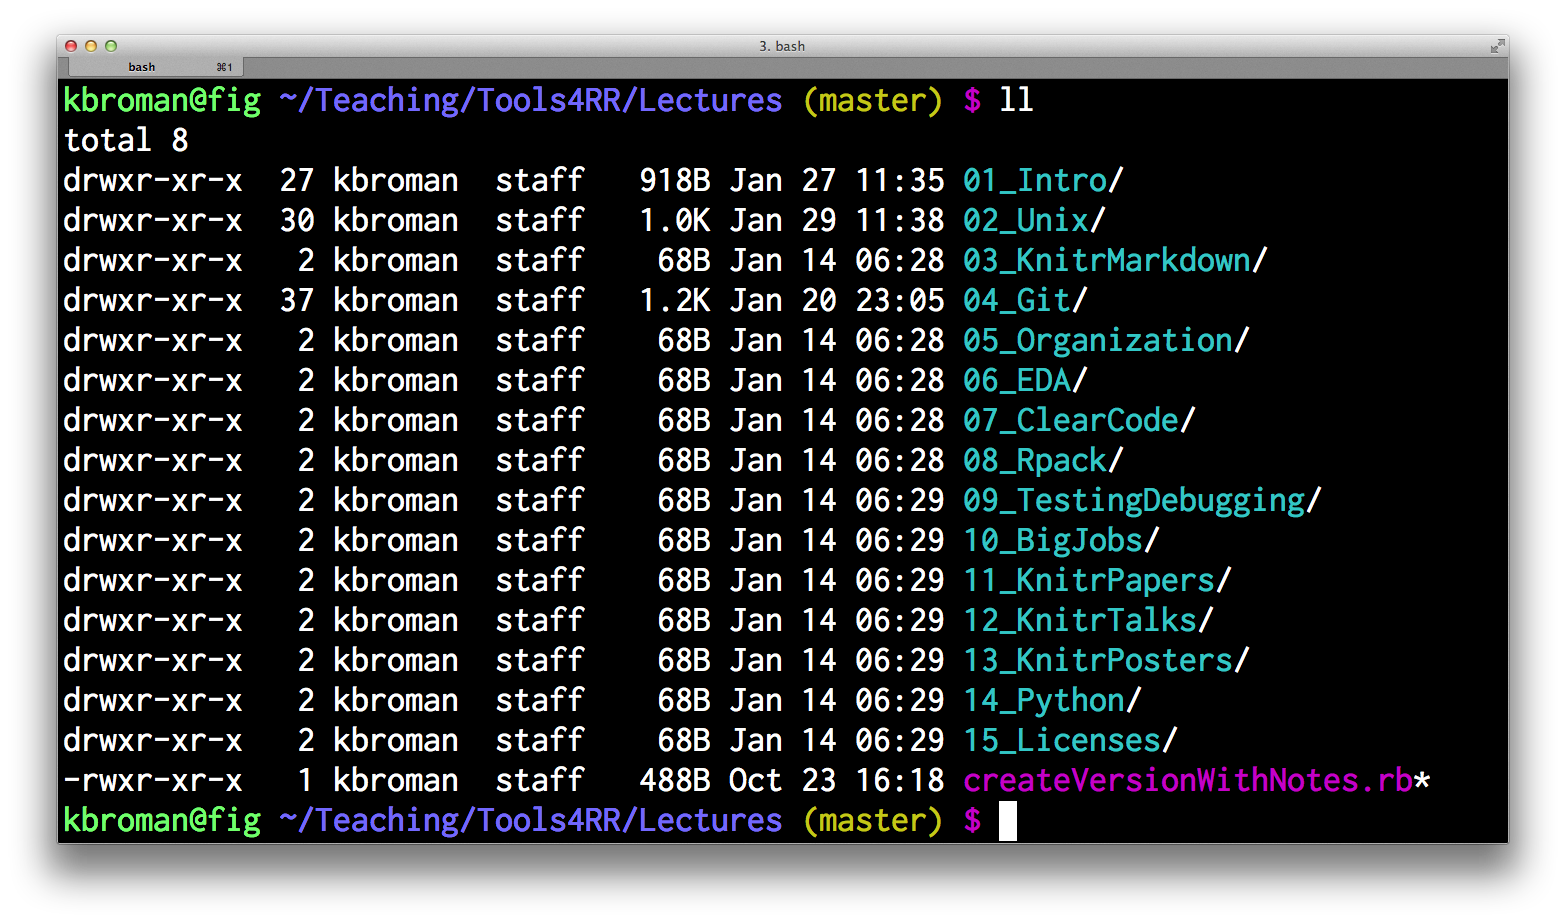
\includegraphics[width=\textwidth]{Figs/chmod.png}}

\note{Note the mode, owner, and group for each file.

mode = read/write/executable for owner/group/everyone}

\end{frame}


\begin{frame}{File modes/owner/group}

\vspace{24pt}

\tt sudo chown kbroman .

chgrp -R staff .

chmod +x createVersionWithNotes.rb

chmod 755 02\_Unix

chmod 644 02\_Unix/02\_unix.tex

chmod 700 Private\_stuff

\note{You don't usually need to change the owner or group assigned to
  a file or directory, but it's good to be aware of the possibility.

  You often want to make scripts executable, or make files/directories
  unreadable. The octal codes (e.g, 755 and 644) are convenient, once
  you get the hang of them.}

\end{frame}


\begin{frame}{How to solve computing problems}

\vspace{24pt}

\bi
\item {\color{vhilight} Try stuff!}
\item man pages and help files
\item {\tt blah -h} or {\tt blah --help}
\item \href{http://www.google.com}{Google}
\item \href{http://stackoverflow.com}{Stackoverflow}
\item \href{http://www.google.com}{Google} with {\tt site:stackoverflow.com}
\item email lists and google groups
\item friends or colleagues
\item \href{http://twitter.com}{Twitter}
\ei

\note{It's surprising how many computing problems can be solved by
  googling the error message.

  You will run into crazy and mysterious errors. Will you give up, or
  figure them out?
}
\end{frame}


\begin{frame}{Examples}

\vspace{24pt}

\bi
\item How do you suppress warnings in knitr?
\item What symbol corresponds to the unicode {\tt \\u00B1}?
\item What's the difference between {\tt curl} and {\tt wget}?
\item What does "{\tt 502 Bad Gateway}" mean?
\item "{\tt To open gs you need to install X11}"
\item {\tt mclapply} isn't working in Windows
\item How to ping a server in Python?
\item {\tt Font shape `EU1/pplx/m/n' undefined}
\ei

\note{These are examples of things you might search for.

If you don't understand an error message, start by pasting it into
google.
}
\end{frame}


\begin{frame}[c]{Important principle}

\centerline{Learn to code by looking at good code.}

\note{Identify programmers that you respect (e.g., Hadley Wickham),
  and study what they do.
}
\end{frame}



\begin{frame}{Choose a good editor}

\vspace{24pt}

\bi
\itemsep12pt
\item \href{http://www.emacswiki.org/emacs/}{Emacs}
\item \href{http://www.vim.org/}{VIM}
\item \href{http://www.rstudio.com/ide/}{RStudio}
\item \href{http://www.barebones.com/products/textwrangler/}{Textwrangler}
\item \href{http://notepad-plus-plus.org/}{Notepad++}
\item \href{http://sourceforge.net/projects/tinn-r/}{Tinn-R}
\ei

\note{I use emacs; I should probably use vim. 

  RStudio is increasingly
  useful, but as a general editor (for things that aren't R), I think
  it's insufficient.
}
\end{frame}


\begin{frame}{A good editor}

\vspace{24pt}

\bi
\itemsep12pt
\item Doesn't require pointing-and-clicking
\item Easy to get code between R and a script
\item Syntax highlighting of code
\item Automatic indentation
\item Close parentheses/brackets/braces
\item Browse code across files
\item Integrated with other tools (e.g., version control)
\ei

\note{I've not figured out how to explore code across a set of files
  in emacs; otherwise I'm very happy with it.
}
\end{frame}


\end{document}
